% =====================================================================
%  Domain-Complete Intelligence  --  two-column arXiv-style position note
%
%  BUILD:   make          (or: latexmk -pdf main.tex)
%  CLEAN:   make clean
%
%  This is a DRIVER file. It contains no prose. To contribute, edit the
%  section files in  sections/  and the bibliography in  references.bib.
%  Style lives in  preamble.tex ; title/authors in  metadata.tex .
% =====================================================================
\documentclass[twocolumn,10pt]{article}
% arXiv: force the pdflatex route (recommended when using pdflatex + TikZ figures)
\pdfoutput=1

% =====================================================================
%  preamble.tex  --  shared style for the DCI position note
%  Edit style HERE (once), not inside section files.
% =====================================================================
\usepackage[utf8]{inputenc}
\usepackage[T1]{fontenc}
\usepackage[margin=0.75in,columnsep=0.28in]{geometry}
\usepackage{amsmath,amssymb,amsfonts}
\usepackage{bm}
\usepackage{booktabs}
\usepackage{array}
\usepackage{microtype}
\usepackage{xcolor}
\usepackage{times}
\usepackage{titlesec}
\usepackage{caption}
\usepackage[numbers,sort&compress]{natbib}
\usepackage{tikz}
\usetikzlibrary{arrows.meta,positioning,calc,fit,backgrounds}
\usepackage[colorlinks=true,allcolors=black,citecolor=NavyBlue,urlcolor=NavyBlue,linkcolor=NavyBlue]{hyperref}

% ---- named colours -------------------------------------------------
\definecolor{NavyBlue}{RGB}{0,64,128}
\definecolor{RuleGrey}{RGB}{90,90,90}

% ---- section heading style (compact, arXiv-ish) --------------------
\titleformat{\section}{\normalfont\large\bfseries}{\thesection}{0.6em}{}
\titleformat{\subsection}{\normalfont\normalsize\bfseries}{\thesubsection}{0.6em}{}
\titlespacing{\section}{0pt}{1.2ex plus 0.4ex minus 0.2ex}{0.6ex plus 0.2ex}
\titlespacing{\subsection}{0pt}{1.0ex plus 0.3ex minus 0.2ex}{0.5ex plus 0.2ex}

% ---- caption style -------------------------------------------------
\captionsetup{font=small,labelfont=bf,labelsep=period,skip=4pt}

% ---- table helpers -------------------------------------------------
\newcolumntype{L}[1]{>{\raggedright\arraybackslash}p{#1}}
\renewcommand{\arraystretch}{1.15}

% ---- semantic macros (keep notation consistent across contributors)
\newcommand{\DCI}{\mbox{DCI}}
\newcommand{\NWAP}{\mbox{NWAP}}
\newcommand{\Dom}{\mathcal{D}}          % the domain
\newcommand{\Rule}{\mathcal{R}}         % the executable rule substrate / verifier
\newcommand{\Prin}{\Pi}                 % the vertically organizing principle
\newcommand{\Snw}{S_{\mathrm{NW}}}      % network-weighted action
\newcommand{\etap}{\eta^{2}_{p}}        % partial eta-squared
\newcommand{\dQ}{\Delta Q}
\newcommand{\arxivid}[1]{\href{https://arxiv.org/abs/#1}{arXiv:#1}}

% ---- tighten lists a touch -----------------------------------------
\usepackage{enumitem}
\setlist{leftmargin=1.4em,itemsep=0.2ex,topsep=0.4ex}

% ---- misc ----------------------------------------------------------
\setlength{\parskip}{0.2ex}
\frenchspacing

% =====================================================================
%  metadata.tex  --  title, authors, affiliations, date
%  New contributors: add yourself to the author block below.
% =====================================================================
\newcommand{\PaperTitle}{Domain-Complete Intelligence:\\[2pt]
\large The Missing Rung Between Reasoning and Universal Agency}

\newcommand{\PaperSubtitle}{A position note}

\newcommand{\AuthorBlock}{%
  Martin G. Frasch\textsuperscript{1,2}\,\href{https://orcid.org/0000-0003-3159-6321}{\small\textsuperscript{[ORCID: 0000-0003-3159-6321]}}
  \quad\textperiodcentered\quad
  Jim Schwoebel\textsuperscript{2,3}\\[4pt]
  \small \textsuperscript{1}Health Stream Analytics, LLC \textperiodcentered\ University of Washington (IHDD)\\
  \small \textsuperscript{2}Task Force for AI Agents in Healthcare \textperiodcentered\ \textsuperscript{3}Quome Inc.\\
  \small \texttt{martin@hsa.bio}%
}

% Keywords line (shown under the abstract; arXiv has no keywords field, so this lives in the PDF)
\newcommand{\PaperKeywords}{artificial general intelligence; skill-acquisition efficiency;
  verifier-guided discovery; action principles; world models; neural architecture search;
  philosophy of science}


% ---- title block ---------------------------------------------------
\title{\vspace{-3.2em}\bfseries \PaperTitle\\[4pt]
       \normalsize\normalfont\itshape \PaperSubtitle}
\author{\AuthorBlock}
% For an internal draft, swap the next line for:
%   \date{\small\today\ \textperiodcentered\ Draft --- not for distribution}
\date{\today}

\begin{document}
\twocolumn[
  \begin{@twocolumnfalse}
    \maketitle
    \begin{abstract}
      \noindent The ARC-AGI program frames the escalation beyond Level~2 (fluid reasoning) as a step toward \emph{universal} agentic intelligence. We argue that this skips a rung that is both more tractable and, for the near term, more consequential for humanity: \textbf{Domain-Complete Intelligence (\DCI)} --- agents that autonomously acquire \emph{any} skill or discovery derivable within a domain whose dynamics are generated by a verifiable rule substrate, but that do not claim generality across domains. We define \DCI\ as a specific, deliberate configuration of Chollet's own measure of intelligence: maximal skill-acquisition efficiency over a constrained scope, purchased by injecting a maximally compressed, scale-invariant prior --- a \emph{vertically organizing principle} $\Prin$ --- together with an executable verifier that supplies closed-loop ground truth. We show that the standard objection to any domain-bounded intelligence (that the meta-skills of discovery seem to require cross-domain generality) is answered \emph{within} the framework, provided $\Prin$ is reflexive across the object/meta boundary. The \mbox{Emin/Imax} neural-architecture-search results are the existence proof of that reflexivity. The upshot: \textbf{Kepler-class agents before Newton-class ones.} Much of the accessible near-term scientific value lies on the earlier rung.

    \end{abstract}
    \vspace{0.4em}
    {\small\noindent\textbf{Keywords:} \PaperKeywords\par}
    {\small\noindent\textbf{ACM classes:} I.2.0 (Artificial Intelligence, General); I.2.6 (Learning).\par}
    \vspace{1.0em}
  \end{@twocolumnfalse}
]

\section{The gap in the Level 2 $\rightarrow$ Level 3 escalation}
\label{sec:gap}

ARC-AGI-3 defines the step beyond static reasoning as \emph{agency}: an interactive benchmark scoring a system's efficiency at acquiring new skills through exploration, model formation, goal inference, and planning --- explicitly probing adaptation to ``unknown unknowns'' \citep{arcprize2026,cholletarc2026}. The framework treats this as continuous with the pursuit of universal generality --- the eventual goal being an agent competent across arbitrary, unseen domains.

We propose that the escalation is mis-cut. Between Level~2 and universal agentic AGI there is a distinct, characterizable rung: agents that are \emph{complete within a domain} --- able to reach, autonomously and by closed-loop discovery, any skill or law derivable from the domain's generative rules --- without any claim to cross-domain transfer. We call this \textbf{Domain-Complete Intelligence (\DCI)}, by analogy to Turing-completeness: not ``can do everything,'' but ``can reach everything derivable within this system.''

This is not narrow AI. Narrow AI has \emph{fixed} skill within a domain (Deep Blue plays chess; it does not discover chess-like regularities in data it has never seen). \DCI\ has open-ended \emph{skill acquisition and discovery} within a domain: it proposes hypotheses, simulates, falsifies, and iterates, reaching competences no designer enumerated in advance. By \emph{discovery} we mean, operationally, the capacity to propose, test, falsify, and retain models or skills \emph{not enumerated at design time} --- the property that separates \DCI\ from advanced optimization over a fixed, pre-specified space (a distinction we make precise in \S\ref{sec:cross}). Its generality is complete \emph{relative to the domain's rule system} and empty outside it. Every genuinely superhuman discovery system built to date --- AlphaFold \citep{jumper2021}, AlphaGeometry \citep{trinh2024}, FunSearch \citep{romera2024} --- is domain-complete-with-a-verifier, not general. That is not a limitation of those systems; it is the shape of the rung.

\section{Definition in Chollet's notation}
\label{sec:definition}

Chollet defines the intelligence of a system as skill-acquisition efficiency over a scope of tasks, controlling for generalization difficulty, priors, and experience \citep{chollet2019}:
%
\begin{equation}
I_{\mathrm{IS},\,scope}
=\underset{T\in scope}{\mathrm{Avg}}
\!\left[
\omega_{T,\theta}\!
\sum_{C\in Cur^{\theta}_{T}}\!
P_{C}\cdot
\frac{GD^{\theta}_{T,C}}
{P^{\theta}_{\mathrm{IS},T}+E^{\theta}_{\mathrm{IS},T,C}}
\right]
\label{eq:chollet}
\end{equation}
%
with $GD$ generalization difficulty, $P$ priors, $E$ experience, $\omega$ the value/difficulty weight, and $C$ a curriculum. (Structure faithful to \emph{On the Measure of Intelligence}; subscripting simplified.)

\textbf{\DCI\ is a configuration of this same functional}, not a different measure. It is defined by four simultaneous constraints:

\begin{enumerate}
\item \textbf{Bounded scope.} The scope is restricted to a domain $\Dom$ whose dynamics are generated by a rule substrate $\Rule$.
\item \textbf{Executable verifier.} $\Rule$ is \emph{executable}: it returns ground truth for any proposed skill or discovery. This drives the cost of experience $E$ toward the cost of computation, because the agent can propose--simulate--falsify--iterate with no human in the loop.
\item \textbf{Compressed prior.} The prior $P$ is dominated by a single, maximally compressed principle $\Prin$ --- ideally a physics-/first-principles action functional. The concrete instance used here is the \textbf{Network-Weighted Action Principle (\NWAP)}, which posits that biological, neural, and law-discovery systems all extremize $\Snw = \int (E - I + A\!\cdot\!C)\,dt$ --- energy minimization $E$, information maximization $I$, and a connection-cost penalty $A\!\cdot\!C$ \citep{frasch2026a,frasch2026b,frasch2026c}. In Chollet's currency (intelligence as compression), such a first-principles law is the extreme point: the most compressed prior available for a physical domain, hence the largest achievable $P$. Its empirical signature --- a \emph{fall in the training energy} required to learn under the objective --- is a direct measurement of elevated skill-acquisition efficiency in Chollet's exact sense (lower $E$ for equal $GD$).
\item \textbf{Verticality.} $\Prin$ is \emph{scale-invariant} --- a \emph{vertically organizing principle} in the sense of \citet{frasch2026a}: a law invariant across levels of organization, as opposed to scale-specific (``horizontal'') causality. Its form is preserved across the levels of organization within $\Dom$.
\end{enumerate}

\DCI\ is therefore the region of Chollet's Pareto frontier where \textbf{acquisition efficiency is maximized by trading breadth for verifiable depth}: large $P$ (from $\Prin$), cheap $E$ (from $\Rule$), over deliberately narrow scope. This is a Chollet-\emph{native} claim, not a departure from his definition.

\section{The verifier is load-bearing}
\label{sec:verifier}

What distinguishes a rule substrate from mere structure is that it closes the discovery loop. In open-world settings there is no oracle, so ``agentic'' behavior degrades into plausible-sounding action with no falsification signal. An executable $\Rule$ converts \emph{agentic} from a vibe into a testable loop: the agent's proposals are adjudicated by the domain itself. This is precisely what universal AGI lacks and cannot cheaply acquire, and precisely what every superhuman discovery system to date has possessed.

The literal demonstration is already in hand. Under a triple-action functional --- trajectory reconstruction ($I_{\max}$), architectural sparsity ($E_{\min}$), and energy-conservation enforcement ($\mathcal{L}_{\mathrm{Symmetry}}$, grounded in Noether's theorem) --- the Minimum-Action Learning (MAL) system selects the correct symbolic force law from a candidate basis on noisy orbital data: it recovers the inverse-square (Kepler) and linear (Hooke) laws, returning the Kepler third-law exponent as $p = 3.01 \pm 0.01$ at roughly a $40\%$ reduction in training energy versus prediction-error-only baselines, with an energy-conservation criterion discriminating the true law where short-term fit alone cannot --- lifting a $40\%/90\%$ direct-selection rate to $100\%$ pipeline-level identification \citep{frasch2026b}. (A wide-stencil preprocessing step cuts noise variance ${\sim}10^{4}\times$, turning an $\mathrm{SNR}\approx 0.02$ problem into a learnable one at ${\approx}\,1.6$.)

Crucially --- and this is a \emph{feature} for the present argument, not a caveat --- the paper is explicit that MAL is a model-\emph{selection} framework over a specified basis, not an open-ended discovery system. This locates MAL precisely: it instantiates the \emph{selection} facet of domain-completeness (reaching the correct law within a given rule library), while the fuller facet --- extending the library \emph{within the domain's own generative grammar} --- is the remaining step. Both are domain-bounded; neither is universal. That boundedness is exactly the \DCI\ signature: completeness \emph{relative to a rule substrate} (here, the basis library and the conservation law that adjudicates it), not open-ended universal discovery. A domain-complete discovery loop closing against a physics substrate is what the Keplerian rung (\S\ref{sec:positioning}) looks like when instantiated --- and its principled boundedness is the point, not a shortfall.

\section{The cross-generality objection --- and why $\Prin$ answers it}
\label{sec:cross}

\textbf{Objection.} Some skills \emph{within} a domain --- experiment design, tool orchestration, recognizing when the data violate the domain's rules --- appear to require cross-domain generality. If so, \DCI\ is not a clean stepping stone but a partial one.

\textbf{Resolution.} The objection conflates two axes that a vertically organizing principle separates. Verticality answers each on different grounds.

\emph{Epistemic axis (cross-scale transfer and violation detection).} Because $\Prin$ is the scale-invariant of $\Dom$, a rule-violation \emph{is} a measurable departure from $\Prin$: an invariant is, by construction, the object whose violation is diagnostic. No external reasoner is required to flag it. Likewise, transfer across scales is not bolted on --- it is constitutive of holding $\Prin$ at all, since $\Prin$ has the same form at every level. The effective scope of a $\Prin$-grounded \DCI\ is thus the \emph{entire vertical hierarchy} $\Dom$ spans, not a thin slice of it. Most of the ``isn't this just narrow AI'' reflex dissolves here.

\emph{Pragmatic/meta axis (search, experiment design, orchestration).} These are not cross-scale but meta-level, and scale-invariance alone does not cover them. They are covered by a further, substantive property: \textbf{$\Prin$ is reflexive across the object/meta boundary} --- it governs not only the dynamics of $\Dom$ but the dynamics of \emph{discovery over} $\Dom$. If skill acquisition is itself an action-minimizing trajectory, then experiment design is ``select the path through hypothesis space that minimizes network-weighted action,'' an instance of $\Prin$ at the meta-level rather than a separate faculty demanding external generality.

This reflexivity is not asserted; it is demonstrated, and along two independent routes (Figure~\ref{fig:reflexivity}) --- with the neural-architecture paper \citep{frasch2026c} supplying the engineering proof of the first and the formal basis of the second.

\emph{Instance 1 --- reflexivity through search.} The \textbf{Emin/Imax} formalism maps \NWAP\ onto neural architecture design: an energy-first objective (the action functional) evaluated across \textbf{2{,}203 experiments} spanning vision, text, neuromorphic, and physiological data, with $10$ seeds per configuration and a factorial analysis \citep{frasch2026c}. The \emph{same} principle that describes an object system also governs the \emph{search} for architectures that model it --- a strong architecture$\times$dataset interaction ($\etap = 0.44$) shows the objective selecting task-appropriate structure rather than a fixed winner. Here the meta-level is design over model space, and $\Prin$ governs it.

\emph{Instance 2 --- reflexivity through inference.} \citet{frasch2026c} also places \NWAP\ in the same variational equivalence class as the free-energy principle and the evidence lower bound (ELBO) of Bayesian inference --- three trade-off-based objectives that balance a data-fit term against a coupling/complexity cost. The paper is careful here, and so is this argument: \NWAP\ is \emph{not} a probabilistic ELBO, but a member of the same equivalence class of variational principles. That class-membership is what matters. The ELBO and the free-energy principle are not object-level descriptions; they \emph{are} the operations by which a system infers a generative model of its data. If $\Prin$ shares their variational form, then model-discovery over the domain is governed by an objective of the \emph{same class} as $\Prin$ --- structural kinship at the object/meta boundary, not a loose metaphor and not a claim of literal identity. And this is not only formal: the same action-functional constraint has been validated at biology scale, predicting the emergent modular organization of real marine metabolic networks, with a modularity excess of $\dQ \approx 0.15$--$0.40$ over configuration-model, label-permutation, and bipartite-incidence null models \citep{frasch2026d}. So reflexivity is witnessed both in \emph{search} (in silico, NAS) and in \emph{inference} (empirically, on real data) --- two different meta-level operations, two different evidentiary bases, with \citeyear{frasch2026c} as the shared formal spine.

\begin{figure*}[t]
\centering
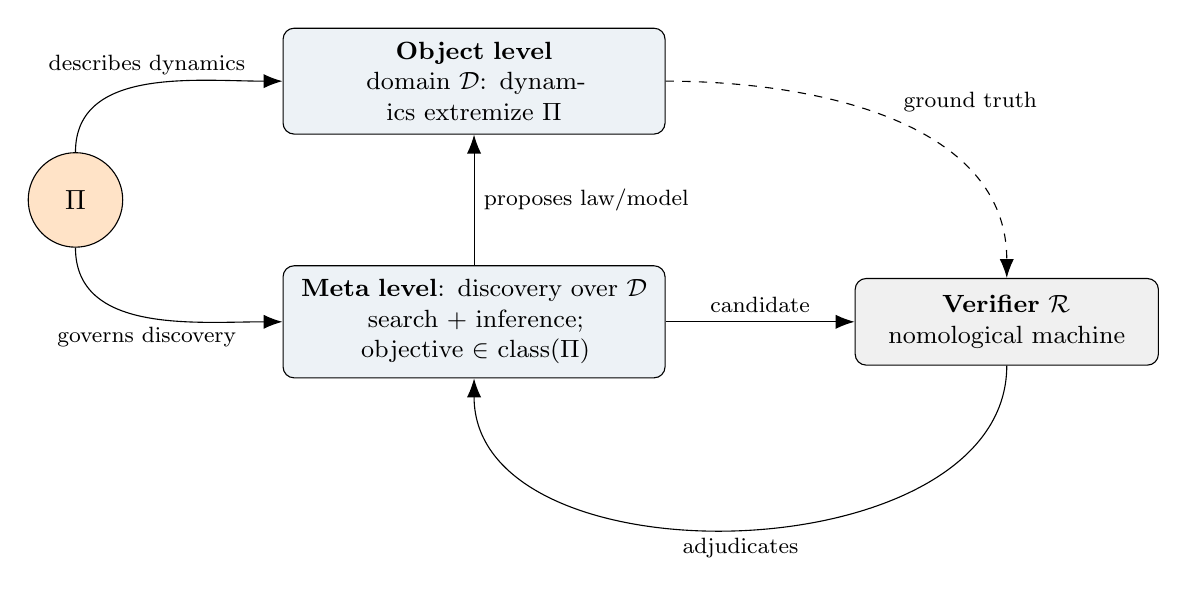
\begin{tikzpicture}[font=\small,>={Latex[length=2.4mm]},
  box/.style={draw,rounded corners,align=center,inner sep=5pt,minimum height=11mm},
  lvl/.style={box,fill=NavyBlue!7,text width=4.5cm},
  ver/.style={box,fill=gray!12,text width=3.5cm},
  prin/.style={draw,circle,fill=orange!22,inner sep=2pt,minimum size=12mm,font=\normalsize}]
\node[prin] (pi) {$\Prin$};
\node[lvl,above right=4mm and 22mm of pi] (obj) {\textbf{Object level}\\ domain $\Dom$: dynamics extremize $\Prin$};
\node[lvl,below right=4mm and 22mm of pi] (meta) {\textbf{Meta level}: discovery over $\Dom$\\ search $+$ inference; objective $\in$ class$(\Prin)$};
\node[ver,right=24mm of meta] (ver) {\textbf{Verifier} $\Rule$\\ nomological machine};
% reflexivity: one principle governs both levels
\draw[->] (pi.north) to[out=90,in=180] node[above,font=\footnotesize]{describes dynamics} (obj.west);
\draw[->] (pi.south) to[out=-90,in=180] node[below,font=\footnotesize]{governs discovery} (meta.west);
% reflexive object/meta coupling
\draw[->] (meta.north) -- node[right,font=\footnotesize]{proposes law/model} (obj.south);
% closed discovery loop against the verifier
\draw[->] (meta.east) -- node[above,font=\footnotesize]{candidate} (ver.west);
\draw[->] (ver.south) to[out=-90,in=-90] node[below,font=\footnotesize]{adjudicates} (meta.south);
\draw[->,dashed] (obj.east) to[out=0,in=90] node[above right,font=\footnotesize]{ground truth} (ver.north);
\end{tikzpicture}
\caption{The object/meta reflexivity loop. A single vertically organizing principle $\Prin$ both \emph{describes} the object-level dynamics of $\Dom$ and \emph{governs} the meta-level discovery over $\Dom$ --- the reflexivity that answers the cross-generality objection. Discovery is witnessed along two routes: Instance~1, search (energy-first NAS, \citealp{frasch2026c}), and Instance~2, inference (\NWAP\ in the free-energy/ELBO variational class, \citealp{frasch2026c}, validated on real data in \citealp{frasch2026d}). The executable verifier $\Rule$ --- a nomological machine (\S\ref{sec:lineage}) --- closes the loop by adjudicating candidates against ground truth, covering any residual the principle does not.}
\label{fig:reflexivity}
\end{figure*}

\textbf{Optimization is not yet agency.} We are careful not to overread the reflexivity evidence, because the object/meta step is where this argument is most easily overstated. Energy-minimization selecting a task-appropriate architecture (Instance~1) is advanced \emph{optimization} over a fixed design space; it is not, by itself, epistemic agency, and we do not claim the NAS result demonstrates the latter. Two meta-skills lie strictly beyond it: (a)~recognizing that the domain's own generative assumptions are wrong --- that it is the rule substrate, not the model, that needs revision --- and (b)~\emph{basis expansion}: inventing a genuinely new term when the existing candidate library cannot express the target law (the open step already flagged in \S\ref{sec:verifier}). What reflexivity actually buys is narrower and still substantive: the \emph{same} objective that scores object-level dynamics also governs search and inference \emph{within a fixed representational basis}. The move from selection to genuine discovery --- basis expansion --- is the sharpest open problem this frame names, not one it claims to have solved. In the interim the executable verifier is what carries discovery across that gap: it makes even an ill-motivated candidate term cheap to falsify, so the mechanism for extending the basis can be dumb (enumeration, mutation, LLM proposal) as long as $\Rule$ adjudicates it. A formal mechanism by which $\Prin$ itself \emph{generates} the missing term remains future work.

\textbf{Composition with the verifier.} Where even these leave residue --- messier real-world meta-skills such as physical experiment orchestration --- the verifier composes with $\Prin$: the executable substrate $\Rule$ substitutes for meta-judgment in exactly the cases where $\Prin$'s meta-coverage is thinnest. Reflexivity of $\Prin$ (search \emph{and} inference) \emph{plus} the verifier substrate together close the loop --- a more robust guarantee than any one of them alone.

The correct statement of the claim is therefore precise, not hand-waving: \emph{a vertically organizing principle addresses the cross-generality concern because it is reflexive across the object/meta boundary; the NAS \citep{frasch2026c} and biology-scale validation \citep{frasch2026d} results are independent evidence that it is; and the verifier substrate covers the residual.}

\section{Positioning: Kepler before Newton}
\label{sec:positioning}

\DCI\ is the \textbf{Keplerian} rung. Kepler mapped mathematical form onto raw observational data to extract laws --- within one domain, with world-historical consequences --- decades before Newton unified the picture. Humanity did not wait for the general theory to reap the value; the domain-complete discovery came first and carried most of the near-term payoff. The analogy is now literal rather than illustrative: a Minimum-Action Learning system recovers the inverse-square gravitational law (and Hooke's) from noisy orbital data and reproduces Kepler's third-law exponent, $p = 3.01 \pm 0.01$, at roughly $40\%$ lower training energy than prediction-error-only baselines \citep{frasch2026b}. We are proposing to build, deliberately, the class of agent that already recovered the Keplerian law from raw data.

Relative to ARC-AGI-3, \DCI\ sits at \textbf{Level 2.5 / Level 3a}: domain-complete agentic intelligence first, open-world agentic intelligence second.

\subsection{Relation to the DeepMind ``Levels of AGI'' taxonomy}
\label{sec:morris}

\citet{morris2024} classify systems on two axes --- \emph{performance} (depth) and \emph{generality} (breadth) --- yielding the matrix in Table~\ref{tab:morris} (representative systems paraphrased from their examples).

\begin{table*}[t]
\centering
\small
\caption{The DeepMind performance$\times$generality matrix \citep{morris2024}, with representative systems. The matrix has no axis for \emph{autonomy of skill acquisition}; that is the dimension \DCI\ adds.}
\label{tab:morris}
\begin{tabular}{@{}L{4.4cm}L{6.0cm}L{5.6cm}@{}}
\toprule
\textbf{Performance $\downarrow$ / Generality $\rightarrow$} & \textbf{Narrow} (task- or domain-specific) & \textbf{General} (wide range of tasks) \\
\midrule
Level 0 --- No AI & calculator; compiler & human-in-the-loop only \\
Level 1 --- Emerging ($\approx$ unskilled human) & simple rule-based systems (classic GOFAI) & frontier chat assistants (early LLMs) \\
Level 2 --- Competent ($\geq$ 50th pct.\ skilled adults) & voice assistants; toxicity classifiers & \emph{not yet achieved} \\
Level 3 --- Expert ($\geq$ 90th pct.) & grammar tools; text-to-image generators & \emph{not yet achieved} \\
Level 4 --- Virtuoso ($\geq$ 99th pct.) & Deep Blue; AlphaGo & \emph{not yet achieved} \\
Level 5 --- Superhuman ($>$ 100\% of humans) & AlphaFold; AlphaZero; Stockfish & \emph{not yet achieved (ASI)} \\
\bottomrule
\end{tabular}
\end{table*}

The reflexive objection to this paper is: \emph{``\DCI\ is just the bottom-left cell --- Superhuman Narrow.''} It is not, and the reason is that this matrix has no axis for \textbf{autonomy of skill acquisition}. Performance measures \emph{how well} a fixed skill is executed; generality measures \emph{how many} task-types are covered. Neither asks whether the system \emph{acquires new skill or discovers new law within its domain on its own}. That question is orthogonal to both, and it is the one that matters for scientific value.

Collapsing that missing axis is exactly what makes ``Superhuman Narrow'' misleading. It houses two categorically different kinds of system (Table~\ref{tab:split}).

\begin{table*}[t]
\centering
\small
\caption{``Superhuman Narrow'' fuses two categorically different kinds of system. \DCI\ is the discovery-capable one, and it is defined by a compressed prior plus an executable verifier rather than by a learned policy.}
\label{tab:split}
\begin{tabular}{@{}L{3.6cm}L{4.6cm}L{7.6cm}@{}}
\toprule
\textbf{Within ``Superhuman Narrow''} & \textbf{Fixed-skill executor} & \textbf{Domain-Complete (\DCI)} \\
\midrule
Example & Stockfish, AlphaZero & AlphaFold-in-a-discovery-loop; AlphaGeometry; FunSearch; the \NWAP\ law-discovery system \citep{frasch2026b} \\
Skill set & fixed at training; superhuman on \emph{one} objective & open-ended \emph{within} the domain's rule system \\
Novelty & executes; does not discover & proposes, falsifies, and reaches un-enumerated results \\
What supplies competence & learned policy & compressed prior $\Prin$ \textbf{+} executable verifier $\Rule$ \\
Failure mode & brittle off-distribution & flags rule-violation as departure from $\Prin$ \\
Empirical anchor (this program) & --- (executes a fixed objective) & law recovered from noisy data, Kepler exponent $p = 3.01 \pm 0.01$ at ${\sim}40\%$ less training energy \citep{frasch2026b}; energy-first design validated across \textbf{2{,}203} experiments, architecture$\times$dataset $\etap = 0.44$ vs.\ architecture-alone $\etap = 0.001$ \citep{frasch2026c} \\
\bottomrule
\end{tabular}
\end{table*}

\DCI\ is therefore \textbf{not a cell but a third axis} --- autonomous discovery --- applied to the deep, narrow, \emph{vertically organized} column. The claim of this paper is that the productive next move is not rightward (toward General, which remains empty at every level above Emerging) but \emph{along this third axis}: promoting narrow-but-deep systems from fixed-skill executors to domain-complete discoverers. And the route runs through explicit, verifiable rule substrates --- through compression via $\Prin$ --- rather than through scale.

\section{Philosophical lineage: \DCI\ and the nomological machine}
\label{sec:lineage}

The frame is not new metaphysics; it is the operationalization of an existing one. Cartwright's \emph{The Dappled World} \citep{cartwright1999} argues that laws of nature are not universal truths holding everywhere and always, but descriptions of the behavior of \textbf{nomological machines} --- stable arrangements of components with fixed capacities that, shielded from interference and set running repeatedly, produce the regular behavior we then codify as law. On this view the world is \emph{dappled}: a patchwork of local regularities, each valid within its machine, not a single seamless deductive system.

Two of this paper's load-bearing commitments are exactly Cartwright's, in computational dress.

First, \textbf{the executable rule substrate $\Rule$ is a nomological machine}. It fixes the components and their capacities, shields the dynamics from outside interference, and can be run arbitrarily many times to generate ground truth. What we called ``closed-loop discovery against a verifier'' is, in Cartwright's terms, an agent operating a nomological machine and reading off its lawful outputs. The verifier is not a convenience; it is the machine that makes lawfulness available at all.

Second, \textbf{\DCI's domain-boundedness is Cartwright's machine-locality, not a limitation to be apologized for}. \DCI\ does not aspire to universal law and then fall short; it aspires to \emph{completeness within a machine}, which on Cartwright's account is where lawfulness genuinely lives. On this view --- a philosophical position, offered as a divergence from the universalist reading rather than a refutation of it --- universality is not so much withheld as reframed: the question ``why isn't this general?'' presupposes that lawful structure is global, whereas a dappled world makes domain-completeness the natural target. This inverts the usual reading of ``narrow'': a domain-complete agent is not a general agent with its scope clipped, but the \emph{natural} epistemic agent for a dappled world. Nothing here forecloses the pursuit of universal agency; the claim is only that the domain-complete rung is real, prior, and where most near-term value sits.

\textbf{Where a domain begins and ends.} Machine-locality invites a fair challenge: if a human must hand-craft the rule substrate $\Rule$ and the token library, is the agent autonomous or merely an efficient search inside a human-built cage? The honest answer distinguishes \emph{provisioning} a machine from \emph{operating} it: supplying $\Rule$ is design, not discovery, and domain-completeness is a claim about what the agent reaches \emph{once} $\Rule$ is fixed, not about inventing $\Rule$ from nothing (the same division of labour that lets us call a scientist creative without crediting them with authoring physics). That division yields three usable boundary criteria, offered as criteria rather than theorems. \emph{Individuation}: a domain is the largest region over which a single $\Prin$ stays invariant and $\Rule$ stays executable; the domain \emph{edge} is exactly where $\Prin$ ceases to be conserved, so a domain cannot expand without bound unless a universal invariant exists --- which is just the universalist claim this paper declines. \emph{Non-triviality}: a domain must admit more than one law derivable from $\Rule$ --- a generative grammar, not a single fact --- or it collapses into a narrow-AI task with nothing left to discover; the interesting domains sit between these poles. \emph{Composition}: two \DCI\ agents whose domains overlap compose exactly where their invariants are jointly satisfied. Chemical physics, for instance, is the intersection region where both the chemical and the physical $\Prin$ hold; a composite agent is domain-complete over that intersection and no further, and where the two invariants conflict neither agent's guarantee survives. Formalizing these criteria --- an explicit calculus of domain intersection and the conditions under which two $\Prin$ compose --- is future work (\S\ref{sec:testable}).

This also sharpens what $\Prin$ is. A vertically organizing principle is the invariant \emph{of a machine} (or of a family of machines that share it), not a Theory of Everything --- the physics cousin being the Laughlin--Pines ``protectorate,'' a higher organizing principle whose consequences hold within its regime irrespective of the underlying microphysics \citep{laughlin2000}. The lineage is therefore clean: Cartwright's nomological machines and dappled lawfulness $\rightarrow$ vertically organizing principles as machine-local invariants \citep{frasch2026a} $\rightarrow$ \DCI\ as the artificial agent that is \emph{complete relative to a machine}. Positioning \DCI\ this way reframes the ``why not just push for general AGI?'' reflex at the level of philosophy of science, not only engineering: to the extent that much of the lawful structure worth discovering is machine-local, the agent matched to it is domain-complete, not universal.

\section{Related work: verifier-guided search and world models}
\label{sec:related}

\DCI\ names and unifies a pattern already visible in the most successful discovery systems, and locates what they share and what they lack.

\emph{Verifier-guided search.} FunSearch pairs a generator with a systematic evaluator to discover programs that surpass known results in extremal combinatorics and bin-packing \citep{romera2024}; AlphaGeometry couples a neural proposer with a symbolic deduction engine that checks each step \citep{trinh2024}. In both, the evaluator/deduction engine is exactly the executable verifier $\Rule$: an oracle internal to the domain that adjudicates proposals. The refinement loops that defined recent ARC-AGI progress --- per-task iterative program optimization guided by a feedback signal \citep{cholletarc2026} --- are the same closed loop without a domain prior. \DCI's contribution here is not the loop but the claim that adding a \emph{compressed, vertically organizing} prior $\Prin$ is what turns a verifier loop into a domain-\emph{complete} discoverer, and what supplies the object/meta reflexivity (\S\ref{sec:cross}) that a bare evaluator does not.

\emph{World models.} A parallel tradition learns a model of environment dynamics and plans or ``imagines'' within it \citep{ha2018}. \DCI's object level $\Dom$ is a world model in this sense --- but one whose dynamics are constrained by an explicit action principle $\Prin$ rather than fit tabula rasa from data. This is the load-bearing difference: verifiability and closed-loop discovery come from the principle plus an executable substrate, not from data coverage alone, which is why \DCI\ inherits the compression (small $P$-cost, cheap $E$) that a learned world model must pay for in experience. Where program-search systems supply the verifier but no prior, and world-model agents supply a learned model but no verifier-grade ground truth, \DCI\ is the configuration that holds both --- a first-principles model \emph{and} an executable adjudicator --- and is therefore complete within its machine rather than merely competent within it.

\section{Scope conditions: when the frame degrades}
\label{sec:scope}

\DCI\ is not a universal solvent, and its guarantees are only as strong as its two assets: a compressed vertically organizing principle $\Prin$ and an executable verifier $\Rule$. Both can be partial, and the frame should --- and does --- degrade gracefully and measurably as either weakens. Stating where it fails is part of what makes it falsifiable.

\emph{Weak or absent $\Prin$.} Many domains of interest may not admit a single scale-invariant action functional; much of biology, economics, and social dynamics may offer only regional symmetries, approximate conservation laws, or learned invariants rather than a genuine $\Prin$. There, \emph{reflexivity through inference} (\S\ref{sec:cross}, Instance~2) weakens with it: absent a true $\Prin$, the meta-level objective is no longer guaranteed to share the object-level's variational form, and the object/meta boundary no longer collapses. The frame makes no claim of domain-completeness in this regime; it predicts \emph{partial} completeness in proportion to how much lawful structure $\Prin$ compresses. This is exactly prediction~(ii) of \S\ref{sec:testable}: a domain with no compressible invariant should show no \DCI\ advantage, which is a way to be wrong, not a hedge.

\emph{Weak or approximate $\Rule$.} Where the substrate is only partly executable --- noisy simulators, costly real-world experiments, oracles that return a signal rather than ground truth --- the closed loop leaks: false positives survive verification and the cost of experience $E$ stops being cheap. Here the composition of the two assets (\S\ref{sec:cross}) does the work: $\Prin$'s meta-coverage must bear more weight precisely where $\Rule$ is unreliable, and $\Rule$ must carry more where $\Prin$ is thin. When \emph{both} are weak at once, \DCI\ has no special leverage and collapses toward ordinary narrow AI, or toward the open-world agentic problem it was meant to precede. That boundary is the honest edge of the proposal, not a concealed failure of it.

\emph{Quantifying the leak.} ``Degrades gracefully'' is only honest if the degradation has a stated shape, so we give one. Let the verifier have fidelity $\rho$ --- the probability it adjudicates a proposal correctly, equivalently one minus its false-positive rate on plausible-but-wrong candidates --- and a per-query cost $c$: a perfect executable substrate has $\rho = 1,\ c \to 0$, while a stochastic simulator or a low-throughput physical assay has $\rho < 1$ and $c$ large enough to inflate the effective experience term $E$. Two regimes bound the behaviour. As $\rho \to 1$ and $c \to 0$ the loop is the closed, cheap-$E$ discovery loop of \S\ref{sec:definition}. As $\rho$ falls, wrong laws survive verification and accumulate; below some domain-dependent threshold $\rho^\ast$ their survival rate exceeds the prior's power to suppress them, the adjudication signal is no longer trustworthy, and \DCI\ reduces to standard RL against an expensive, unreliable reward --- the closed loop provides no advantage over model-free trial-and-error. We do not have $\rho^\ast$ in closed form; locating it, and in particular its dependence on the compression of $\Prin$ (a stronger prior should tolerate a weaker verifier, since it needs fewer bits of ground truth to discriminate candidates), is a concrete measurement this program owes and a further way for the frame to be wrong. The physics case gives the intuition and a lower anchor: wide-stencil preprocessing had to lift an $\mathrm{SNR}\approx 0.02$ substrate to ${\approx}\,1.6$ \citep{frasch2026b} \emph{before} the discovery loop closed at all --- direct evidence that a verifier-quality floor exists and that discovery does not occur beneath it.

\emph{The residual burden on reflexivity.} Even granting $\Prin$ and $\Rule$, the reflexivity claim is best-evidenced for search (NAS) and for the variational form of inference; it is weakest for open-ended meta-skills such as designing a genuinely novel experimental apparatus, or recognizing that the domain's rules themselves require revision --- the basis-expansion step flagged in \S\ref{sec:verifier}. We do not claim these are fully covered by $\Prin$. We claim two narrower things: that the executable verifier substitutes for meta-judgment in the cases that matter for discovery, and that whatever remains uncovered is precisely the frontier where \DCI\ shades into the universal-agency problem --- a frontier we are content to leave to that program rather than to overclaim for this one.

\section{Testable commitments}
\label{sec:testable}

The frame is falsifiable, and each prediction already has a first data point in the four-domain program. It predicts that (i)~systems combining a compressed vertical prior with an executable verifier show markedly higher skill-acquisition efficiency --- lower $E$ for equal $GD$ --- than scale-matched general agents on discovery tasks (the ${\sim}40\%$ training-energy reduction in physics law recovery \citep{frasch2026b}; and the energy-first evaluation across 2{,}203 NAS experiments \citep{frasch2026c} are the first measurements); (ii)~discovery quality tracks the \emph{compression} of the injected prior, not model size; and (iii)~$\Prin$-guided search transfers across domains that share the invariant while general search does not --- the cross-modality NAS results \citep{frasch2026c} and the biology-scale modularity-excess replication \citep{frasch2026d} being the first cross-domain data points. Each is a concrete experiment, not a slogan.

\section{Claim}
\label{sec:claim}

What humanity most needs in the near term is not universal AGI but \textbf{domain-complete AGI}: agents that master discovery on raw data by holding a verifiable, vertically organizing principle and closing the loop against the domain itself. This rung is more tractable than universal generality, more consequential in the near term, and --- because it can be built carefully and creatively around explicit first-principles substrates rather than emergent scale --- more governable. Build the Keplers first.


% ---- bibliography --------------------------------------------------
\bibliographystyle{plainnat}
\bibliography{references}

\end{document}
